
\documentclass[../notes.tex]{subfiles}

\graphicspath{{\subfix{../img/}}}

\begin{document}

\section{ECE568 Computer Security}

\subsection{Refresher \& Introduction}

\begin{blockquote}
    I've found that the way that this course is organized does not lend itself well to well-organized headers and notes. Apologies for the train-of-thought style.
\end{blockquote}


Software systems are ubiquitous and critical. Therefore it is important to learn how to protect against malicious actors. This course covers attack vectors and ways to design software securely



\textbf{Data representation}: It's important to recognize that data is just a collection of bits and it is up to us to tell the computer how it should be interpreted. Oftentimes we can make assumptions, for example assume that an int is an int. But what if we end up being wrong about it? 
Many security exploits rely on data being interpreted in a different way than originally intended.
For example,

\begin{listing}[H]
\begin{minted}{c}
unsigned long int h = 0x6f6c6c6548; // ascii for hello
unsigned long int w = 431316168567; // ascii for world
printf("%s %s", (char*) h, (char*) w);
\end{minted}
\caption{An innocent example of where we should be careful about data representation. This prints hello world}
\end{listing}

This courses makes use of Intel assembler.
TLDR:

\begin{itemize}
  \item 6 General-purpose registers
  \item RAX (64b), EAX(32b), AX(16b), AH/AL(8b), etc
\end{itemize}

Note that the stack grows downwards and the heap grows upwards. Stack overflows can occur and can be a source of vulnerability.


GDB offers some tools for examining stacks

\begin{itemize}
    \item \texttt{break}: create a new breakpoint
    \item \texttt{run}: start a new process
    \item \texttt{where}: list of current stack frames
    \item \texttt{up/down}: move between frames
    \item \texttt{info frame} display info on current frame
    \item \texttt{info args}: list function arguments
    \item \texttt{info locals}: list local variables
    \item \texttt{print}: display a variable
    \item \texttt{x} display contents of memory
\end{itemize}

\begin{itemize}
    \item \texttt{fork}: Creates a new child process by duplicating the parent. The child has its own new unique process ID
    \item \texttt{exec}: Replaces the current process with a new process
\end{itemize}

\marginnote{The fork-exec technique is just a pair of \texttt{fork} and \texttt{exec} system calls to spawn a new program in a new process}

\subsection{Software Code Vulnerabilities}


Recall: the stack is used to keep track of return addresses across function calls; storing a breadcrumb trail.
Another key thing sitting in the stack are local variables. 
A common theme in the course is that computing tends to conflate execution instructions with data.

Common data formats and structures create an opportunity for things to get confused (and for attackers to take advantage of). 
For example, a buffer-overflow attack can end up overwriting that return address breadcrumb trail and then execute arbitrary code.

\begin{figure}[H]
    \centering
    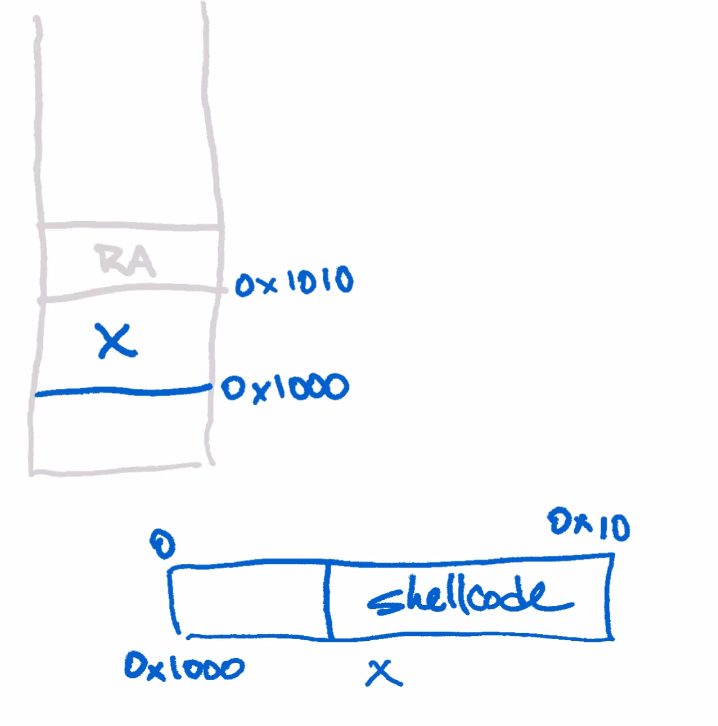
\includegraphics[width=0.8\linewidth]{img/image_2023-01-16-18-27-59.png}
    \caption{Bufferoverflow to write to the return address. Shellcode is a sequence of instructions that is used as the payload of an attack. It si called a shellcode because they commonly are used to start a shell from which the attacker can do more.}
\end{figure}


There are ways to find out where that return address is (or at least reasonably guess).
This is discussed more in detail later; for now we'll assume that they have it figured out.


A common technique to make this easier is to inject a bunch of \texttt{NOP}s before the start of the shellcode. So that we don't need to be as precise as needed in order to find the shellcode start.

One technique for finding the RA would be to incrementally increase the size of the buffer overflow until we get a segfault -- at this point the segfault would tell you what memory address it was trying to access and possibly the values it saw there instead as well.

\begin{figure}[H]
    \centering
    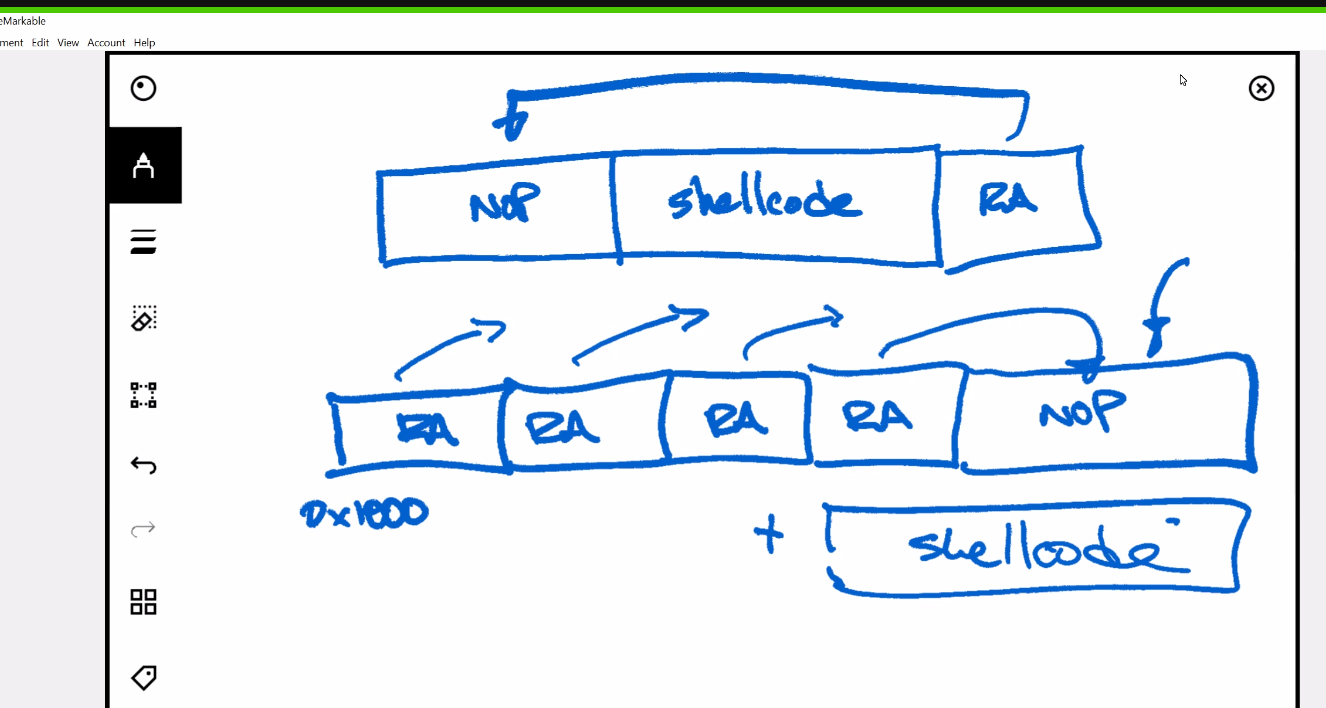
\includegraphics[width=0.8\linewidth]{img/image_2023-01-16-18-37-29.png}
    \caption{Can create a RA sled with a NOP leading to shellcode and then try it from e.g. 0x1000, 0x2000 and so forth to find where to attack from.}



\end{figure}

\begin{figure}[H]
    \centering
    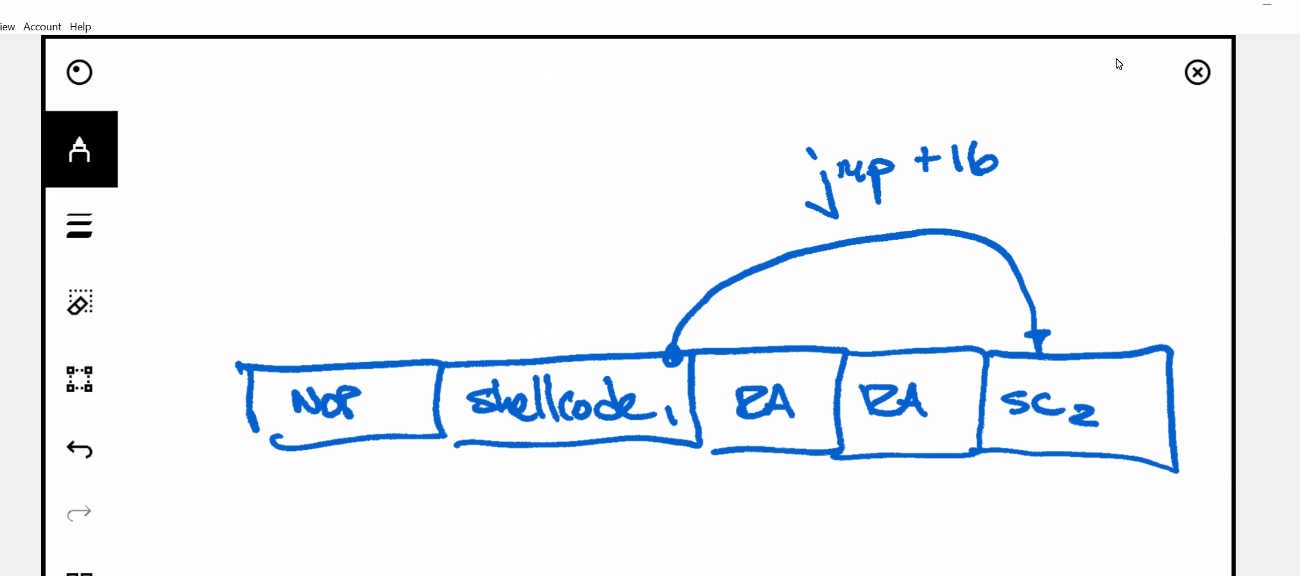
\includegraphics[width=0.8\linewidth]{img/image_2023-01-16-18-40-09.png}
    \caption{Another technique may involve placing shellcode all over the place, of which each one may be a valid entrypoint into the shellcode.}
\end{figure}



\subsection{Format string Vulnerabilities}
\begin{listing}[H]
\begin{minted}{c}
spirntf(buf, "Hello %s", name);
\end{minted}
\end{listing}


\texttt{sprint} is similar to \texttt{printf} except the output is copied into \texttt{buf}. The vulnerability is simiar to the buffer overflow vulnerability. The difference is that the attacker can control the format string.

Consider the following:

\begin{listing}[H]
\begin{minted}{c}
char* str = "Hello world";
printf(str); // 1
printf("%s", str); // 2
\end{minted}
\end{listing}

Despite it looking different there are differences in these two ways to print hello world.
The first argument is a format string, which is different from just a parameter.
A format string contains both instructions for the \texttt{c} printing library as well as data.
This means that the first method can be exploited if the attacker has access to the format string.
A more complex vulnerability is with \texttt{snprintf} (which limits the number of characters written into buf).



\begin{listing}[H]
\begin{minted}{c}
void main() {
    const int len = 10;
    char buf[len];
    snprintf(buf, len, "AB%d%d", 5, 6);
    // buf is now "AB56"
}
\end{minted}
\end{listing}

\begin{itemize}
    \item Arguments are pushed to the stack in reverse order
    \item snprintf copies data from the format string until it reaches a \%. The next argument is then fetched and outputted in the requested format
    \item What happens if there are more \% parameters than arguments? The argument pointer keeps moving up the stack and then points to values in the previous frame (and could actually look at your entire program memory, really)
\end{itemize}

\begin{listing}[H]
\begin{minted}{c}
void main () {
    char buf[256];
    snprintf(buf, 256, "AB,%08x,%08x,%08x,%08x,%08x,%08x,%08x,%08x,%08x,%08x", 5);
    printf(buf);
    // AB,00000005,00000000,29ee6890,302c4241,2c353030,30303030,39383665,32346332,33353363,30333033%                                                                                                                  
    // if we look at the 3rd clause as ascii we get '0,BA' (recall intel little endian) i.e. we've read up far enough to see the local variable specifying the format string pushed onto the stack earlier
}
\end{minted}
\end{listing}
\begin{figure}[H]
    \centering
    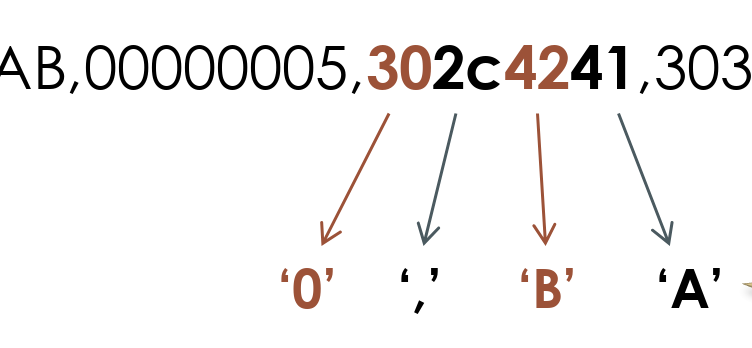
\includegraphics[width=0.8\linewidth]{img/image_2023-01-16-19-06-48.png}
    \caption{ASCII decoding}
\end{figure}

Now there's a potential problem: information leakage (of important info further up the stack).
Programmers may not pay attention to sanitizing input like language config.


\begin{itemize}
    \item \texttt{\%n}: Assume then next argument is a pointer and then it writes the number of characters printed so far into that pointer. 
    \item This can be abused by \%n  write to the return address and then overwrite it with the address of the shellcode.
\end{itemize}


How an exploit may look like for this is as follows:

\begin{figure}[H]
    \centering
    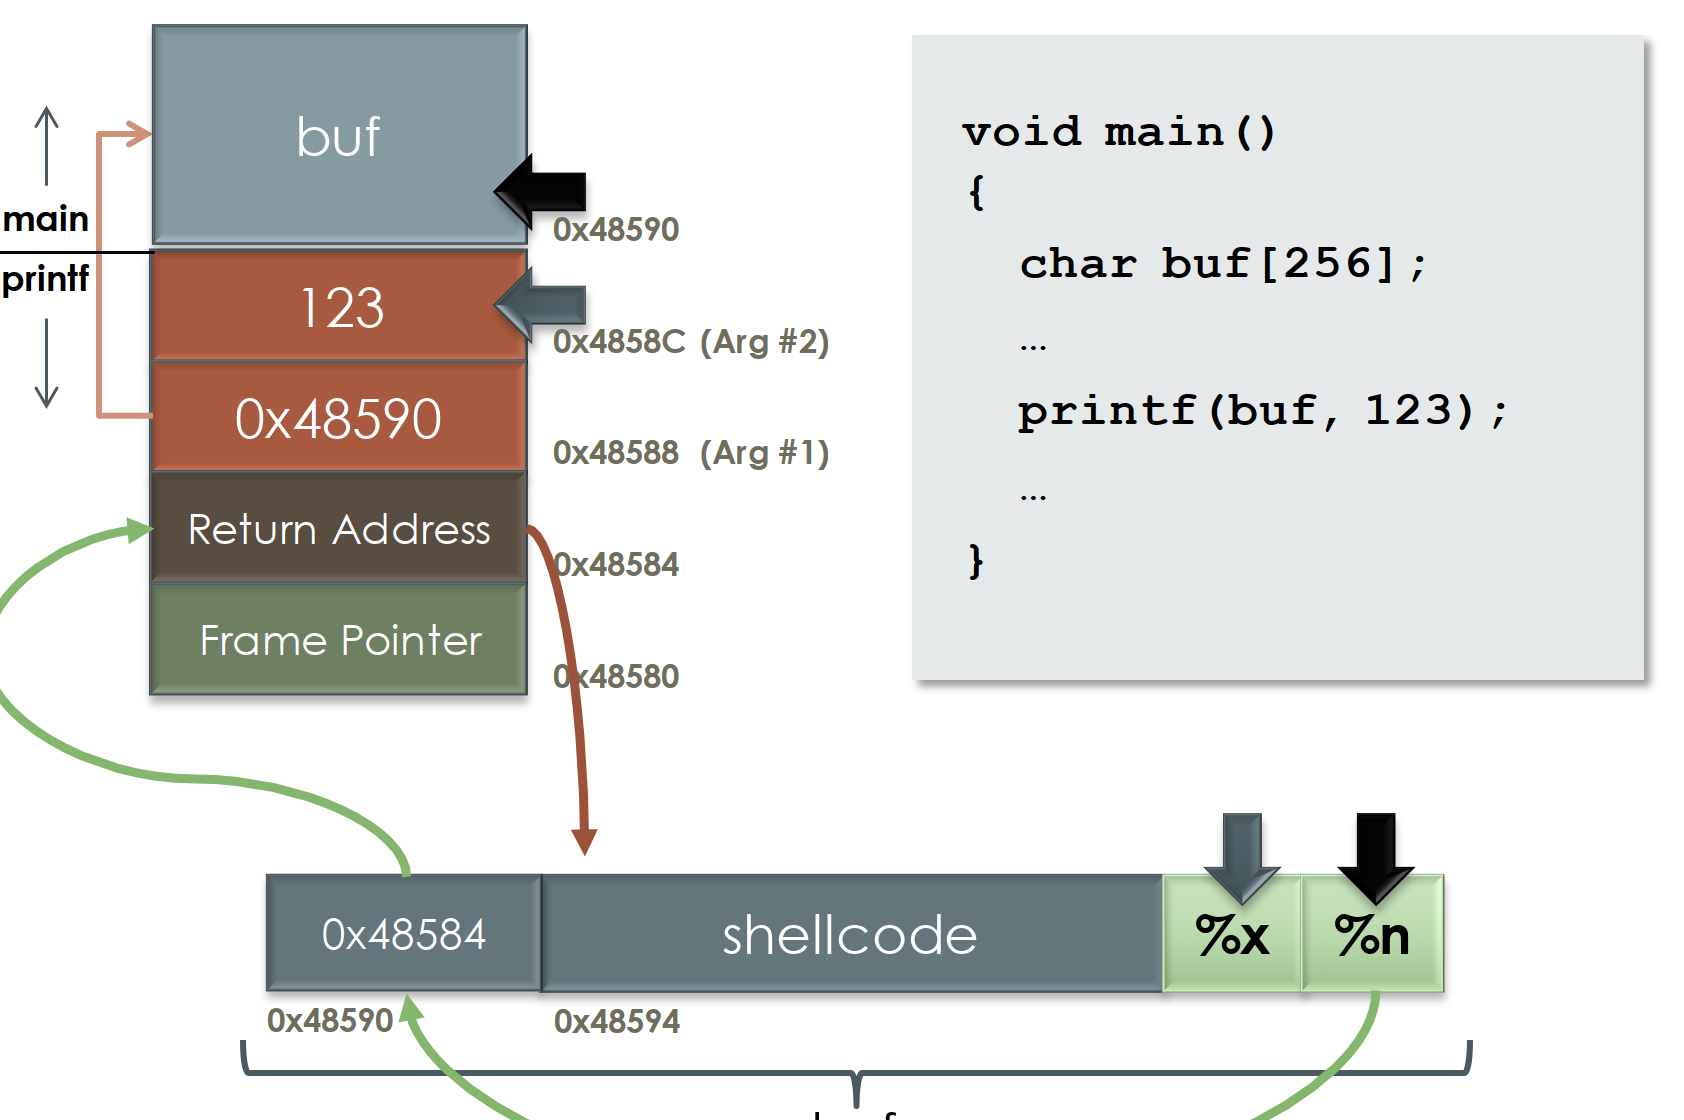
\includegraphics[width=0.8\linewidth]{img/image_2023-01-16-19-39-16.png}
\end{figure}

\begin{enumerate}
    \item Consume the 123 argument (\%x)
    \item Have the return address sitting in the beginning of the memory
    \item Overwrite the RA value with the start of shellcode
\end{enumerate}

There are some problems with this because on modern machines addresses are very large and it can be impractical to create a gigabyte-sized buffer.
Instead we can just divide the problem up and write multiple 8 bit numbers

\begin{figure}[H]
    \centering
    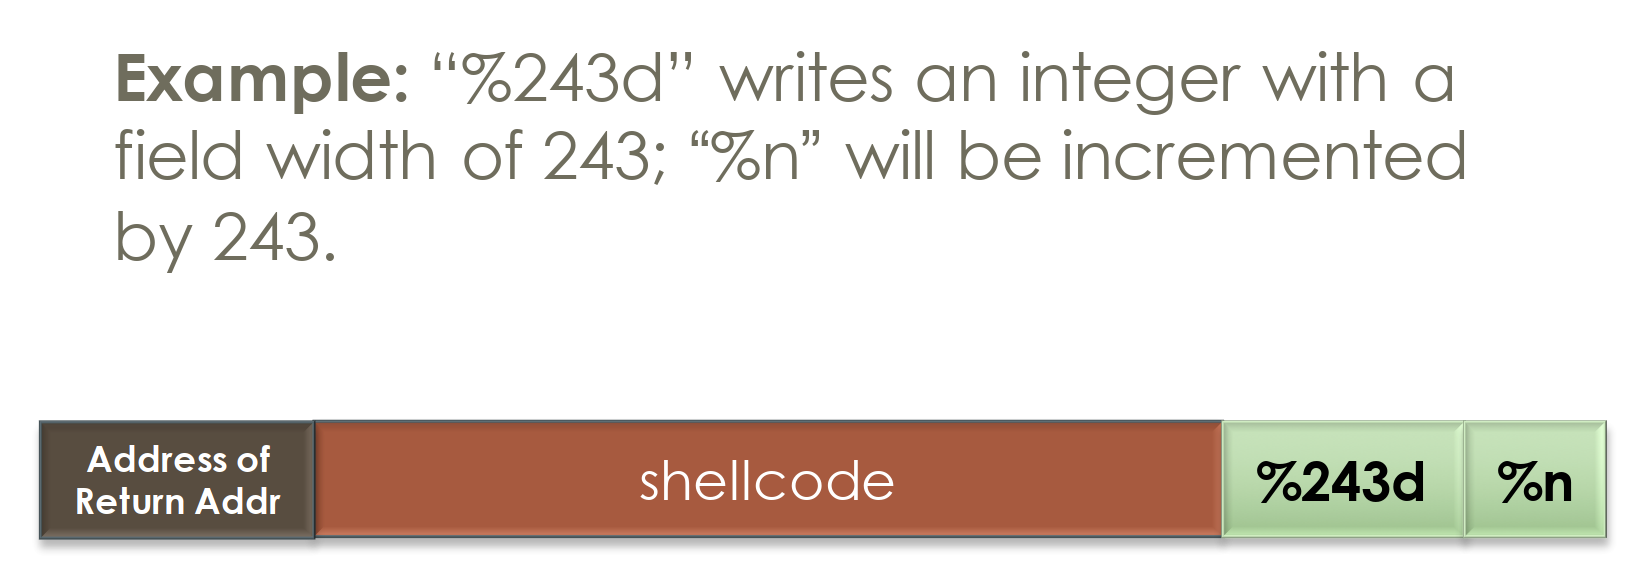
\includegraphics[width=0.8\linewidth]{img/image_2023-01-16-19-46-14.png}
    \caption{The printf count increments by 243 with \%243d. Shorthand}
\end{figure}


\begin{figure}[H]
    \centering
    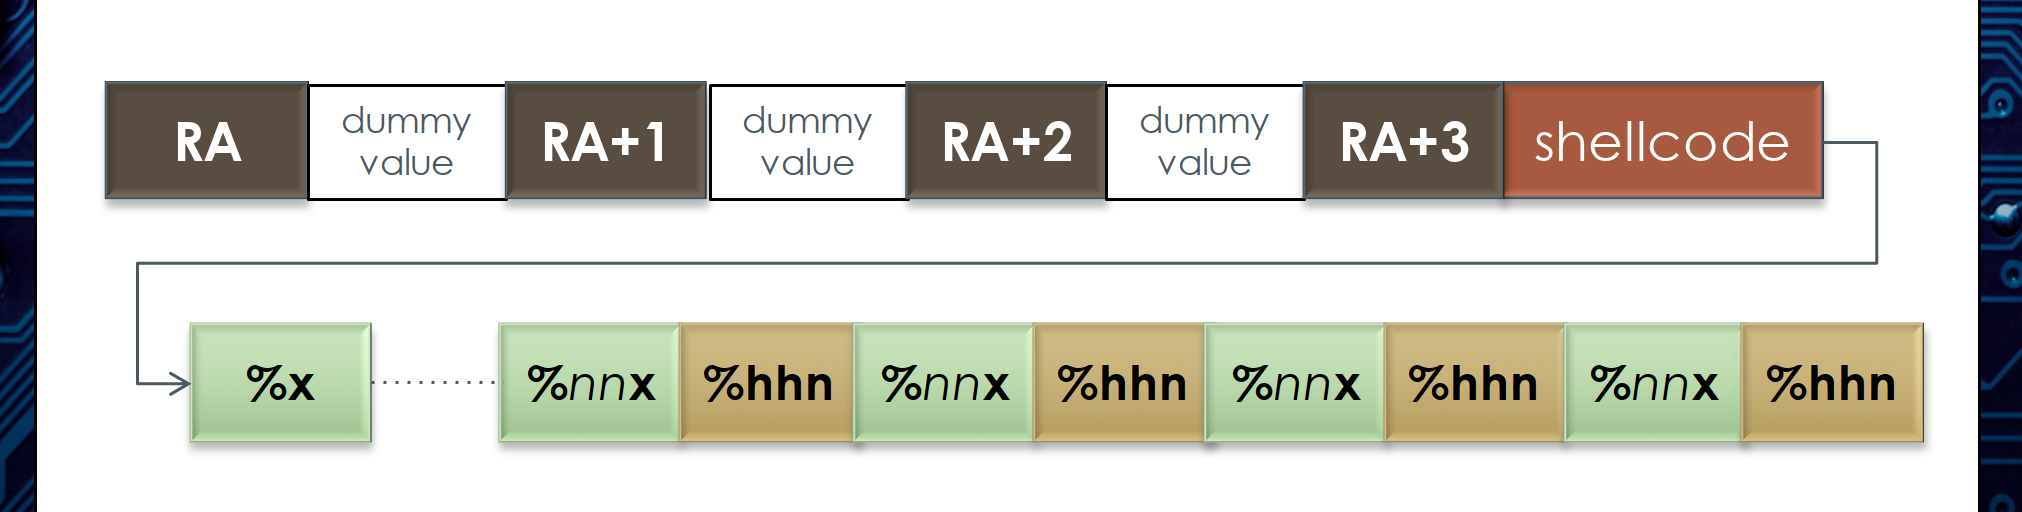
\includegraphics[width=0.8\linewidth]{img/image_2023-01-16-19-48-17.png}
    \caption{The gaps are there because }
\end{figure}
Dividing the problem into pieces; using \%hhn and \%nnx to write 8 bits at a time. \marginnote{Note that this writes the printf counter into the pointer at the argument. This drastically decreases the buffer size needed}

If the bytes being written must be written in decreasing order we can do this by structuring our pointers in a way that we write it in reverse order (don't need to start with LSB). Another option is 



\subsection{Double-Free vulnerability}

Freeing a memory location that is under the control of an attacker is an exploitable vulnerability


\begin{listing}[H]
\begin{minted}{c}
p = malloc(128);
q = malloc(128);
free(p);
free (q);
p = malloc(256);
// this is where the attack happens; the fake tag, shell code, etc
strcpy(p, attacker_string);
free(q);
\end{minted}
\end{listing}

Note that the \texttt{c} free function takes a reference (not necessarily a pointer) to the memory location to be freed. It does not change the value of the free'd pointer either.

\begin{figure}[H]
    \centering
    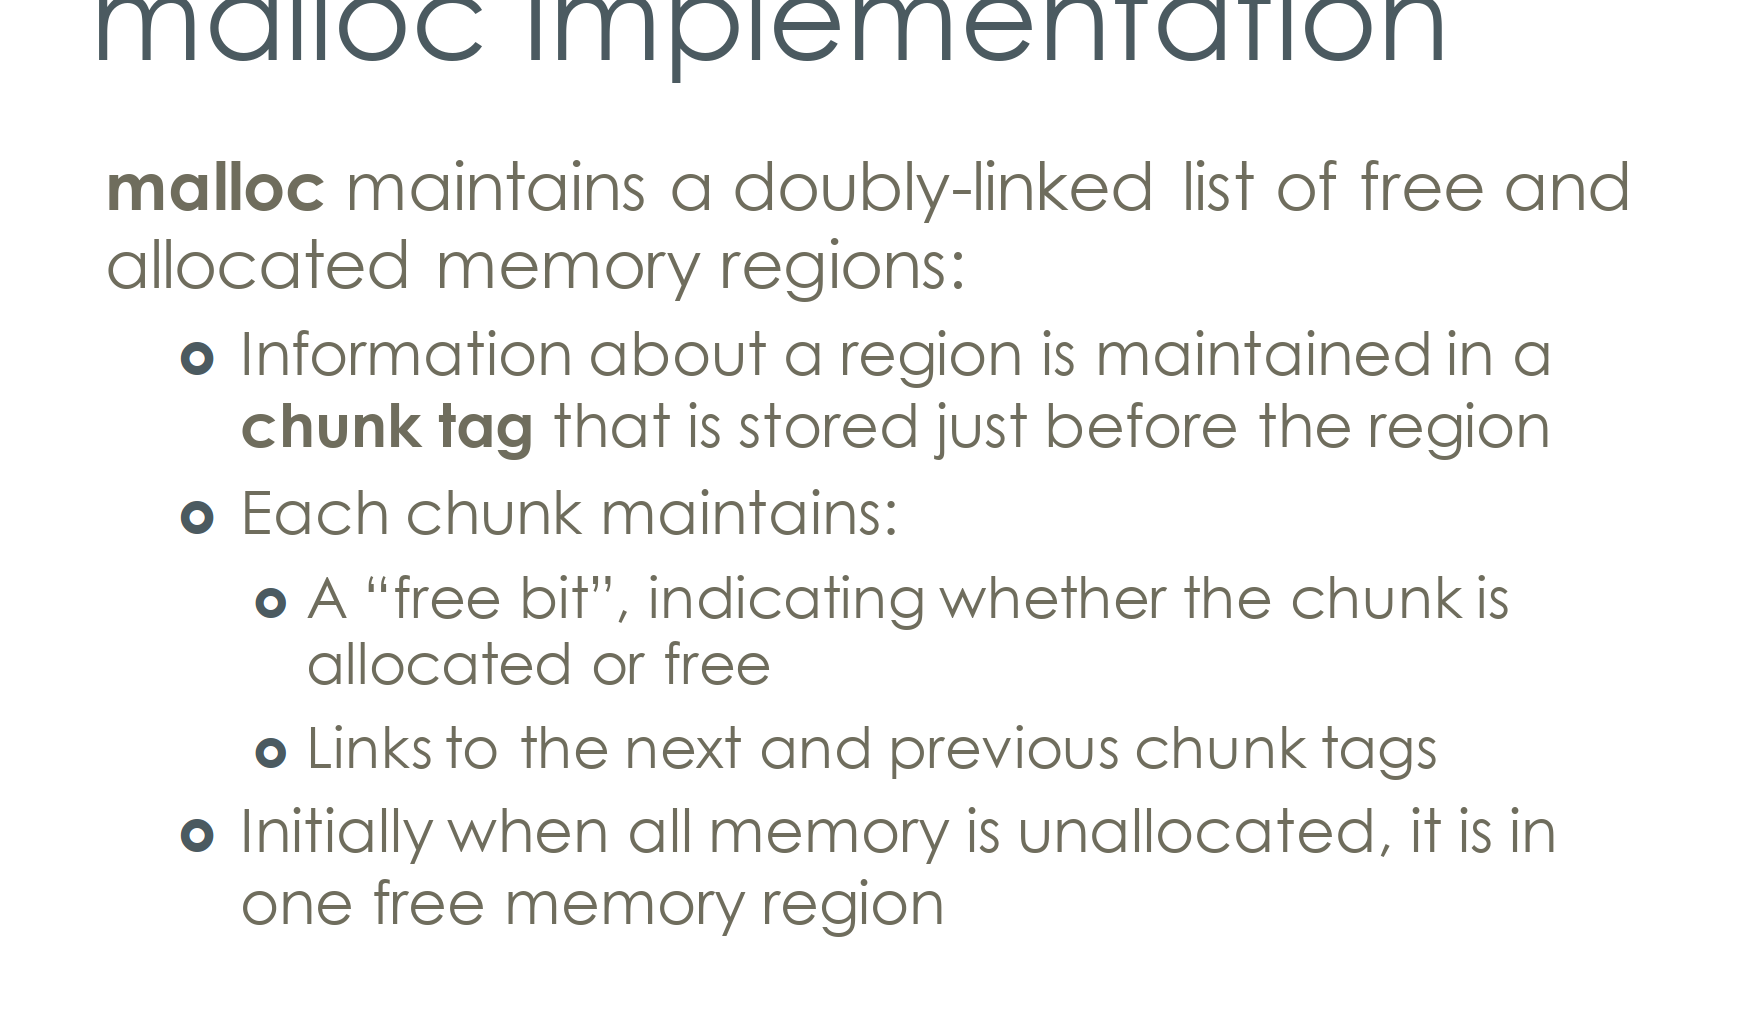
\includegraphics[width=0.8\linewidth]{img/image_2023-01-16-20-08-50.png}
\end{figure}

\begin{figure}[H]
    \centering
    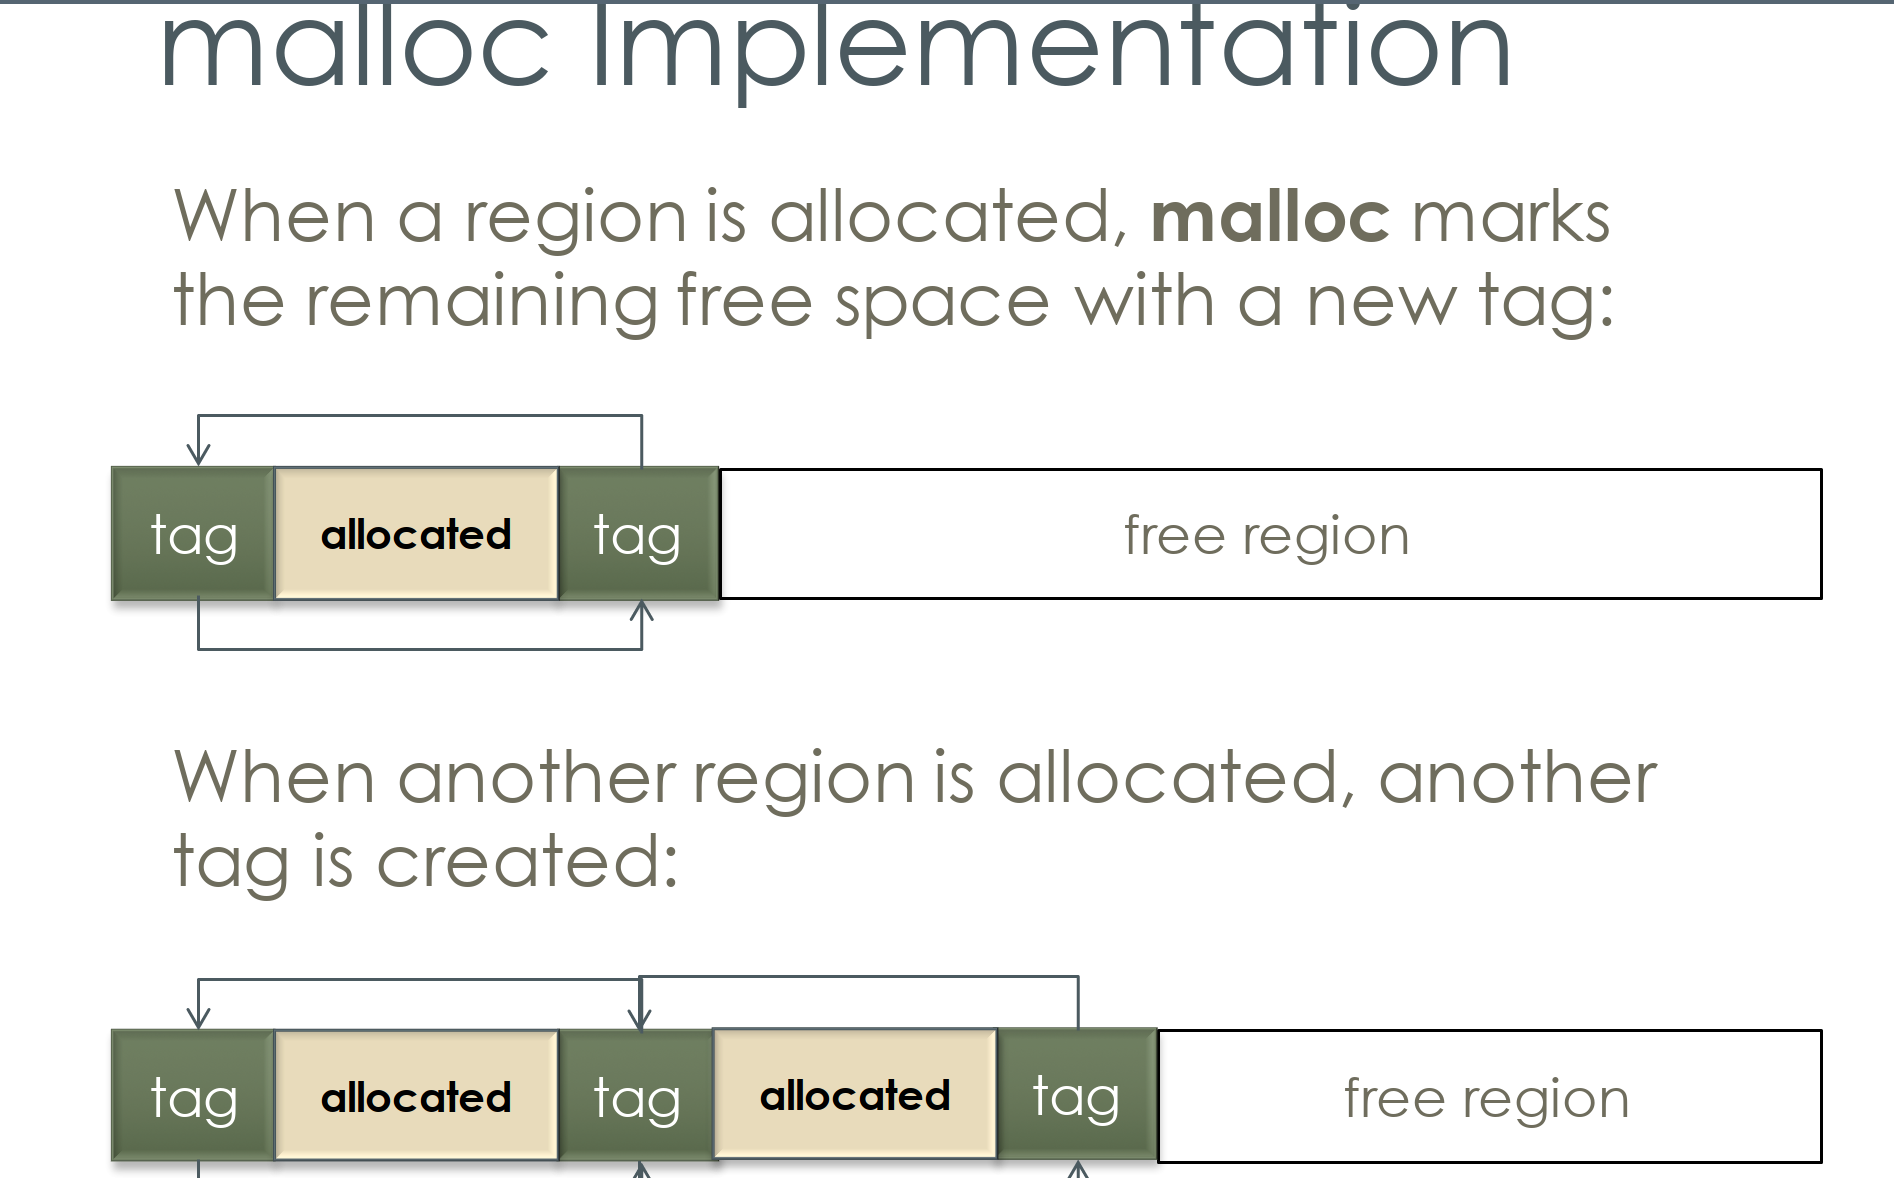
\includegraphics[width=0.8\linewidth]{img/image_2023-01-16-20-09-02.png}
\end{figure}

Malloc places a doubly-linked-list of chunk bits in memory to describe the memory allocated. \texttt{free} sets the free bit, does the various doubly linked list operations (looking at the pointer values of its neighbours in order to remove itself) and also tries to consolidate adjacent free regions.
It assumes that it is passed the beginning of the allocated memory as well as go find the tag associated with the region (which is in a consistent place every time).

The attacker can drop fake tags into memory just ahead of the value we want to overwrite and then we can use the free() call to overwrite memory with the attacker's data.
For example we can create a fake tag node with a prev and next pointer. We make the next pointer be the address of the return address. And then "prev" can contain the address of the start of our shellcode. So freeing on this fake tag will overwrite the return address with the shellcode start.



\begin{blockquote}
    Note that this is not possible with a single free if you are not able to write to negative memory indicies. 
    The part that makes this attack works is that the double free allows the attacker to write a fake tag just before the next tag in a totally valid way. Doing this with a single free would also involve writing to memory that the program doesn't own. (recall: how the memory manager works)
    

\end{blockquote}





\subsection{Other common vulnerabilities}

The attacks we have seen have involved overwriting the return address to point to injecting code. Are there ways to exploit software without injecting code? Yes -- return into \texttt{libc} i.e. use \texttt{libc}'s \texttt{system} library call which looks already like shell code.
This can be accomplished with any of the exploits we have already talked about.

I.e.

\begin{itemize}
    \item Change the return addresses to point to start of the system function
    \item Inject a stack frame on the stack
    \item Before return sp points to $ &system $
    \item System looks in stack for arguments
    \item System executes the command, i.e maybe a shell
\end{itemize}


\begin{itemize}
    \item Function pointers
    \item Dynamic linking
    \item Integer overflows
    \item Bad bounds checking
\end{itemize}


\subsubsection{Attacks without overwriting the return address}

Finding return addresses is hard. So we can use other methods to inject code into the program.

\begin{itemize}
    \item Function pointers: an adversary can just try to overwrite a function pointer
    \item An area where this is very common is with \textit{dynamic linking}, i.e. functions such as \textit{printf}. 
    \item Typically both the caller of the library function and the function itself are compiled to be position independent
    \item We need to map the position independent function call to the absolute location of the function code in the library
    \item The dynamic linker performs this mapping with the procedure linkage table and the global offset table
        \begin{itemize}
            \item GOT is a table of pointers to functions; contains absolute mem location of each of the dyn-loaded library functions
            \item PLT is a table of code entries: onee per each library function called by program, i.e. sprintf@plt
            \item Similar to a switch statement
            \item Each code entry invoes the function pointer in the GOT
            \item i.e. sprintf@plt may invoke jmp GOT[k] where k is the index of sprintf in the GOT
            \item So if we change the pointers in the offset table we can make the program call our own code, i.e. with objdump.\mn{PLT/GOT always appears at a known location.}

        \end{itemize}
\end{itemize}




\subsubsection{Return-Oriented Programming}
\begin{itemize}
    \item An exploit that uses carefully-selected sequences of existing instructions located at the end of existing functions (gadgets) and then executes functions in an order such that these gadgets compose together to deliver an exploit. 
    \item This can be done faster by seeding the stack with a sequence of return addresses corresponding to the gadgets and in the order we want to run them in.
\end{itemize}














\subsubsection{Security Fundamentals}

The three key components of security are:

\begin{itemize}
    \item Confidentiality: the protection of data/resources from exposure, whether it be the content or the knowledge that the resource exists in the first place. Usually via organizational controls (security training), access rules, and cryptography.
    \item Integrity: Trustworthiness of data (contents, origin). Via monitoring, auditing, and cryptography.
    \item Availability: Ability to access/use a resource as desired. Can be hard to ensure; uptime, etc...
\end{itemize}

Together they form an acryonym: CIA. A system is considered secure if it has all three of these properties for a given time.
The strength of cryptographic systems can be evaluated by the number of bits of entropy or their complexity. For example, a 128-bit key has 2\^128 possible values. This would take a lot of time to break, and a 256-bit key even longer.
Availability is harder to measure quantitatively and is instead traditionally measured qualitatively. For example, a system may be available 99.9\% of the time. But this doesn't really measure w.r.t security.


Some security terms:
\begin{itemize}
    \item Another security concept is the \textbf{threat}, or any method that can breach security.
    \item An exercise of a threat is called an \textbf{exploit}  and a successful exploit causes the system to be compromised. Common threats include internet connections/open ports.
    \item \textbf{Vulnerabilities}  are flaws that that weaken the security of a system and can be difficult to detect. For example an unchecked string copy can cause a buffer overflow and allow an attacker to execute arbitrary code
    \item \textbf{Compromises} are the intersection between threats and Vulnerabilities, i.e. when an attacker matches a threat with a vulnerability (i.e. matching a tool in the attacker's arsenal with a weakness)
    \item \textbf{Trust} : How much exposure a system has to an interface. For example a PC might have a lot of trust in the user.
\end{itemize}

The leading cause of computer security breaches are humans. We are prone to making mistakes.
A general trade-off exists when designing secure systems for humans; the more secure a system becomes the less usable it  tends to be. One way of measuring the quality of a security system is how secure it is while maintaining usability

\subsubsection{Reflections on Trusting Trust}

\begin{blockquote}
    \textbf{Reflections on Trusting Trust} is a paper by Ken Thompson that discusses the trust and security in computing. Cool short read.
\end{blockquote}


\begin{figure}[H]
    \centering
    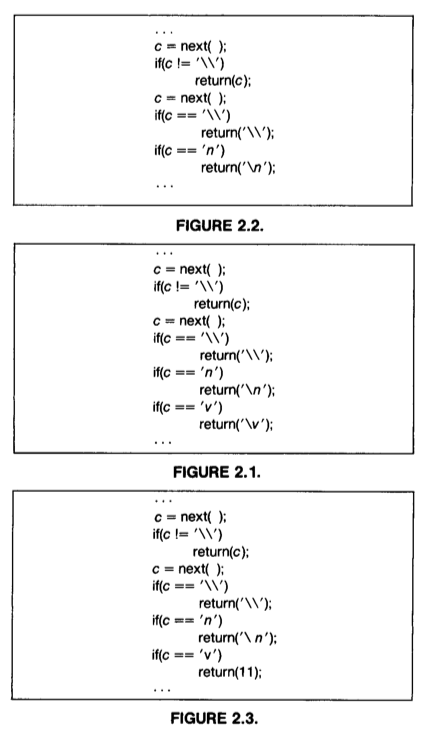
\includegraphics[width=0.8\linewidth]{img/image_2023-01-13-05-03-27.png}
    \caption{Teaching a compiler what the "\textbackslash v" sequence is. We may add a statement to return the ascii encoding of \textbackslash v (11), compile the compiler, and then use it to compile a program that knows what \textbackslash v is. }. We may then alter the source to be like Figure 2.3 without any mention of \textbackslash v but still compile programs with \textbackslash v just fine.
\end{figure}

\begin{figure}[H]
    \centering
    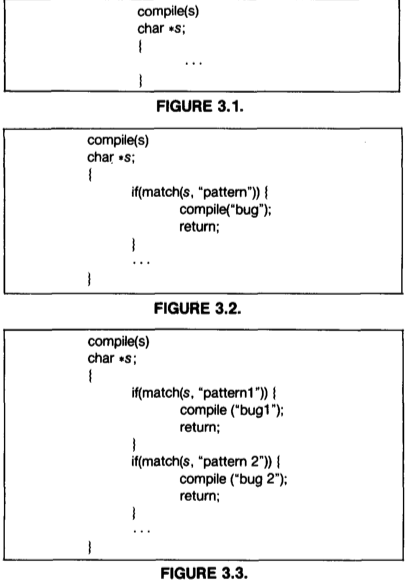
\includegraphics[width=0.8\linewidth]{img/image_2023-01-13-05-08-29.png}
\end{figure}

Next, consider the above scenario where we insert a login Trojan to insert backdoors into code matching the unix login function. We may then compile the $ c $ compiler to do just that, and then change the source to what it should look like without the Trojan. Compiling the compiler one more time will now produce a compiler binary that looks completely innocent but will reinsert the Trojan wherever it can.


The moral of the story is that you can't trust code that you didn't totally create yourself. But it's awfully difficult to use only code written by oneself. So take security seriously.


\end{document}
